% !TEX TS-program = pdflatex


In recent years, the problem of API recommendations rises more and more in relevance in the complex software systems. When a developer writes some code to implement a specific features, he should want some suggestions about useful methods for the library that he is using. Nowadays, a project is not more implemented from scratch but, following the paradigm of software components reuse, developers typical use frameworks, tools, plug-in that make an intensively use of APIs. Their variety depends on the language that the developer use and it usually composed by libraries with objects and methods necessary for the completion of task. This definition is very general and it may change based on the context of the developed project; so, the developer may get confusing about what kind of method or class to use or how to use them in a proper way. Moreover, many APIs are not well described and in many cases documentation miss at all. Although there are forums and dedicated website, as StackOverFlow, with well-organized topic and a lot of code examples, the developer looses its time to search the proper hints for a specific problem. Another aspect to take into account is the fact that each developer have its programming style and so a certain snippet of code could be useful for a user but meaningless for another one. 
\newline
A real big issue is how to perform a good enough recommendation in this context, balancing possible bias and putting the proper hints for the developer. Moreover, the form of the recommendation is also important because, in general, there are variety of possible suggestion such as code snippet, patterns for the methods, enhance documentation and all things that make a recommendation really usable for the current project. In this work, we focus on API function call and we propose a recommendation tool.\\
This work is developed within the European CrossMiner project~\cite{https://www.crossminer.org/_nodate} and integrates some aspect related to the API recommendation domain. As overall aim, the project wants to monitor, analyze and extract data in the context of operative source software (OSS) environment. In this kind of system, there are issues and challenges to be addressed in order to reach a high quality projects, as the choosing of software components to be used during the development. The most difficult part in this task is the searching of the proper software component that is more suitable for the entire projects. Nowadays, the complex software system are really big and it is not so easy to select and deploy a component in the right way. Crossminer wants to face this problem trough various components that address a specific issue relate to the OSS domain, like:
\begin{itemize}
\item Source code analysis tools to extract and store knowledge from the source code of a collection of open-source projects;
\item Natural language analysis tools to extract quality metrics related to the communication channels, and bug tracking systems of OSS projects by using Natural Language Processing and text mining techniques;
\item System configuration analysis tools to collect and analyse system configuration artefacts;
\item Workflow-based knowledge extractors that simplify the analysis of a complex software system;
\item Cross-project relationship analysis tools to manage a wider range of open source project relationships, such as dependencies and conflicts, based on user-defined similarity measures and the creation of project clusters;
\item Advanced integrated development environments that will allow developers to adopt the  knowledge base and analysis tools directly from the development environment, that providing alerts, recommendations, and user feedback which will help developers to improve their productivity.
\end{itemize}
The figure below represents the Crossminer approach, including all issues addressed by the project:\\


\begin{figure}[!h]
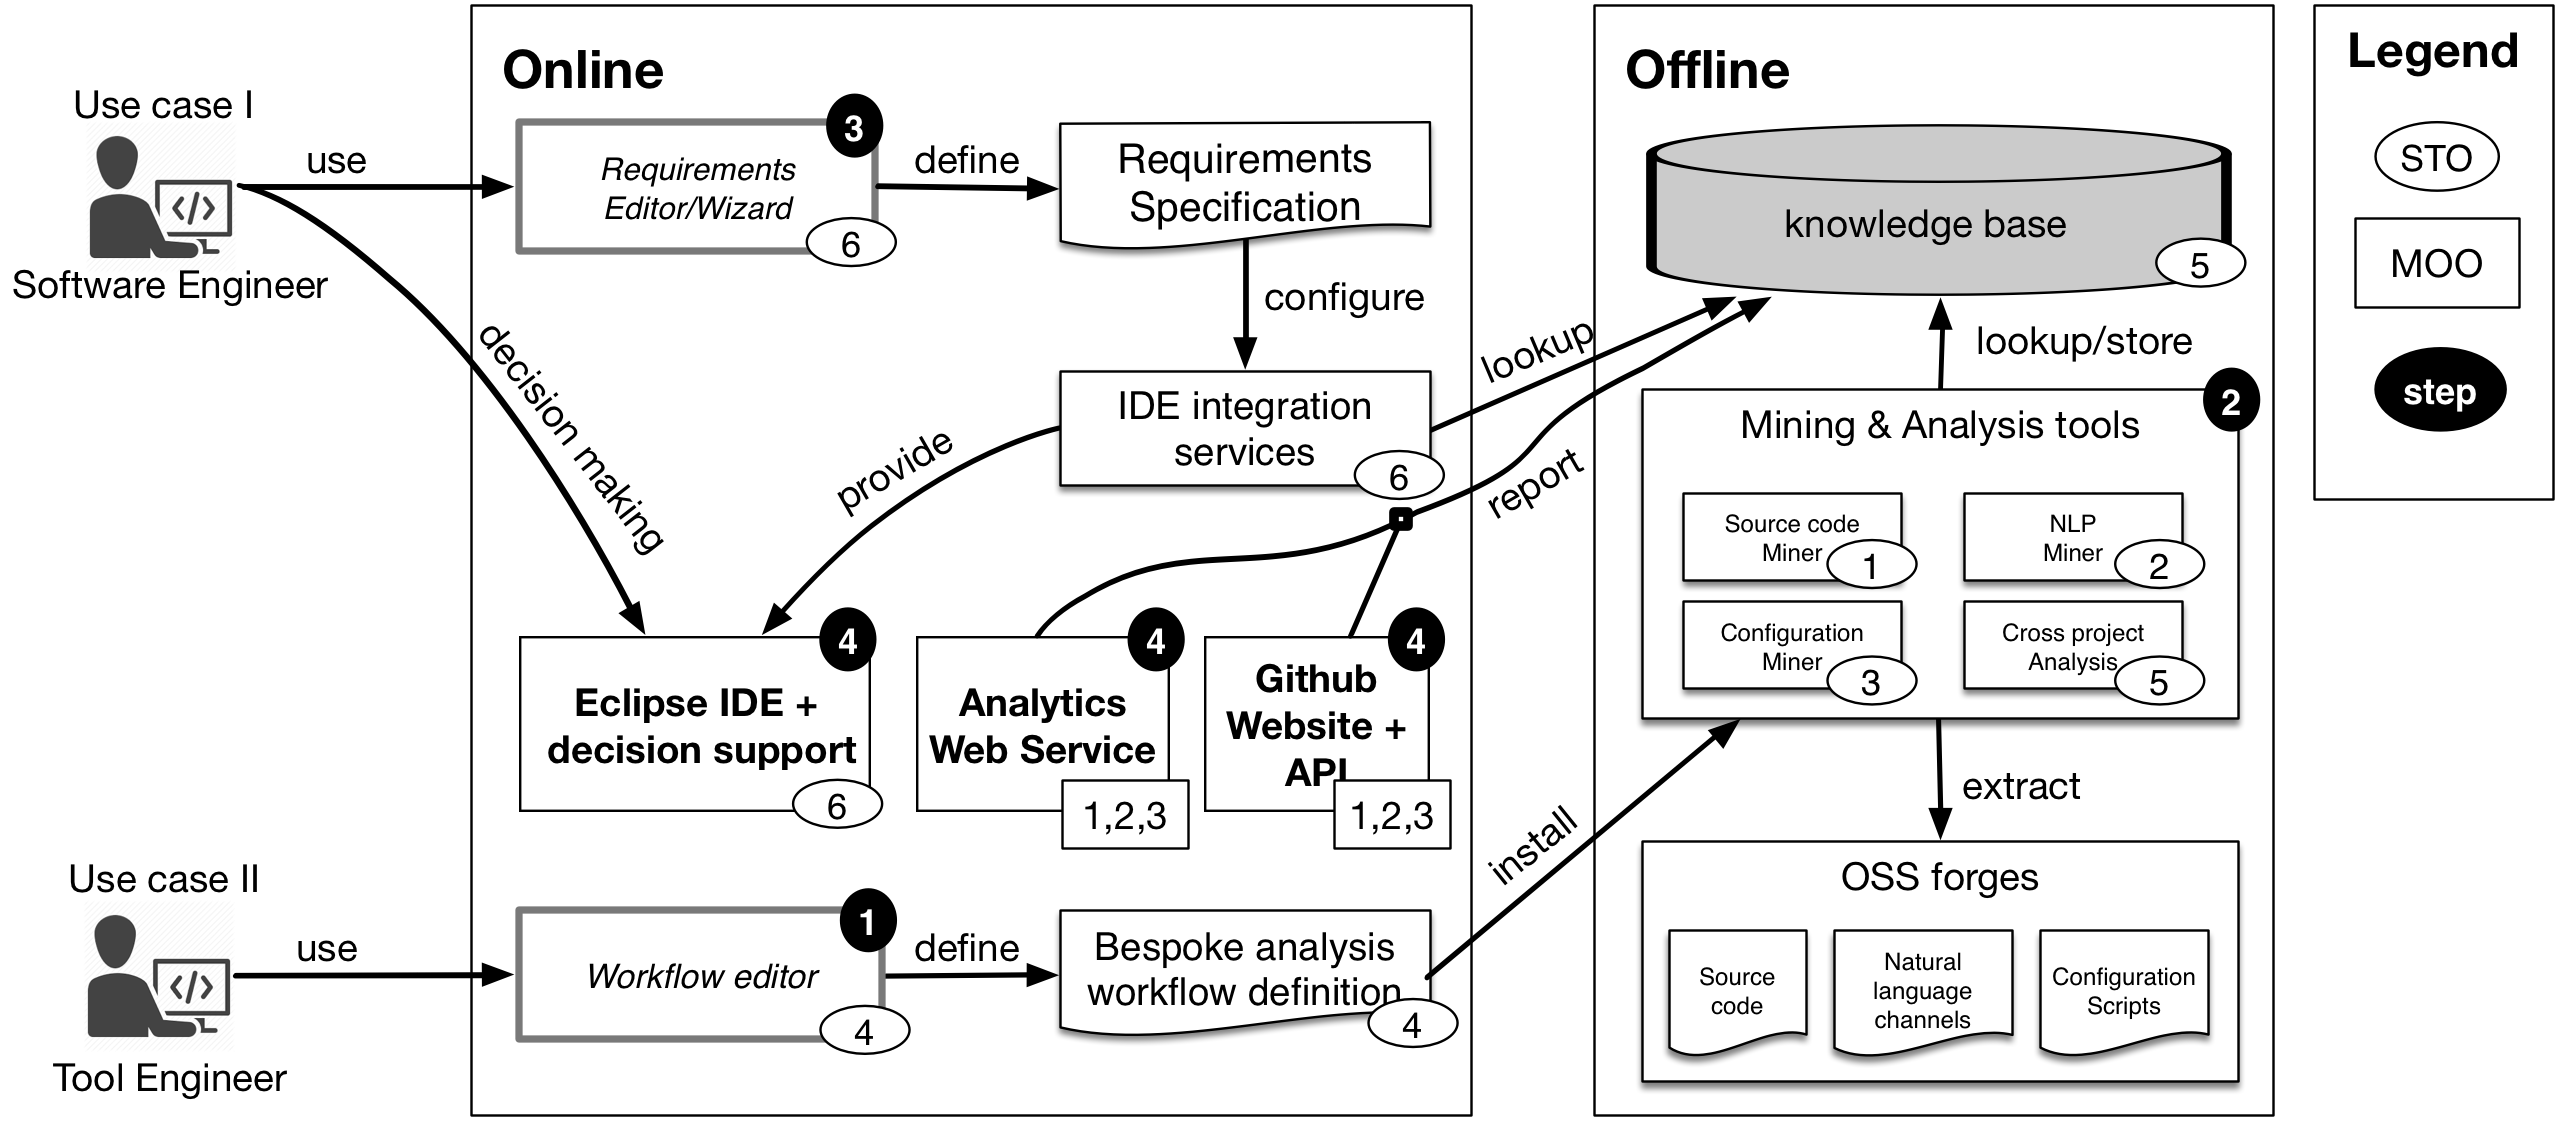
\includegraphics[width=14cm,height=14cm,keepaspectratio]{images/crossminer.png}
\centering
\caption{Crossminer approach}
\label{fig:cmd}
\end{figure}

Among all these challenges, the work presented in this thesis wants to propose a novel tool that perform API function call recommendations in the context of Java projects. It is integrated in the CrossMiner knowledge base component in a flexible way. The figure 1 represents the entire knowledge base; the proposed approach gives support for the APIrecommender subcomponent in the picture.

\begin{figure}[!h]
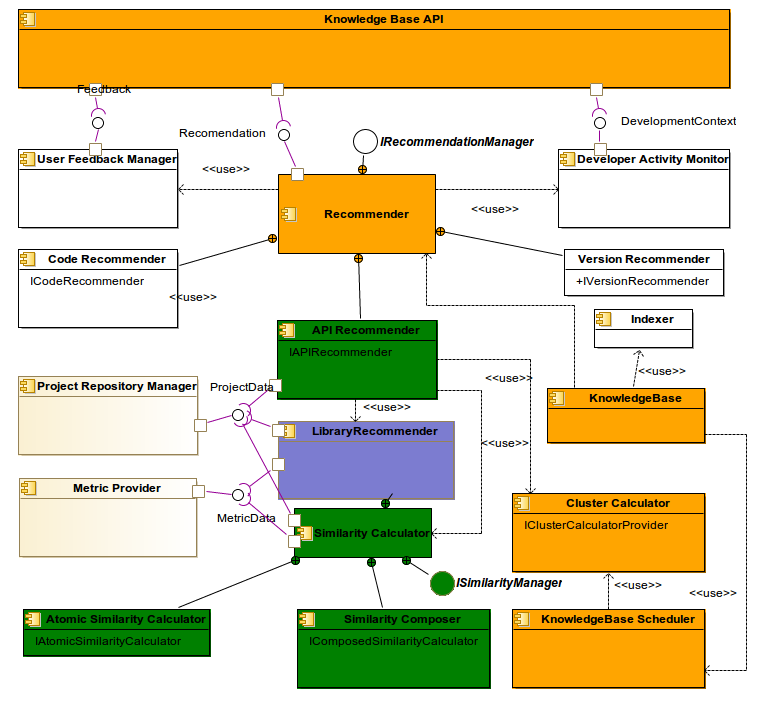
\includegraphics[width=12cm,height=12cm,keepaspectratio]{images/Kb.png}
\centering
\caption{Crossminer knowledge base}
\label{fig:cmd}
\end{figure}

	
In particular, we combine the concepts of code cloning and patterns to retrieve real code snippets that show a concrete usage of the libraries used by the developer. We choose this approach because code snippets represent immediate hints in the developing context, as a concrete usage of a method or class is more relevant rather than a JavaDocumentation description or the list of imports. We exploit also the code cloning technique in order to search and retrieve possible suggestion.\\
The work is organized in this way: in section 2 we provide a general overview on the key concepts used in the developed of the proposed tool. These concepts are the definition of API and recommendation; there are very general terms and the literature are plenty of examples and definitions in such a way that it is impossible to give an exhaustive overview. For this reason, we try to define in the right manner the context suitable for the proposed approach, by avoiding the perfect coverage of the topic and limit ourself to a few but relevant concepts for our aims. Moreover, we provide a general state of the art of the code cloning domain, with some definitions as cloned fragment, sources units and comparison algorithms. We also present different code cloner to have an overview on the different approaches and finally, we present Simian, the code cloner used in the proposed approach.\\
Section 3 gives an overall view of the problem, considering the most used and famous tool used for facing the API recommendation problems. They use very different techniques and a state of the art is necessary to better understand approaches, level of the recommendations and possible issues that arise when we develop these kind of systems.The general API recommendations procedure involves the visit of the AST, some clustering techniques and a ranking as postprocessing phase and we compare various existing approaches. Among these works, we select CLAMS for its results to perform our recommendations and PAM  for validate our approach. \\
The section 4 we describe the proposed tool that perform the final recommendations. It combines the results coming from CLAMS, inserted in the related works section, that are snippets of code representing patterns for a certain library. We use CLAMS as a black box component as it is written in Python (except for slight changes pointed out in the related section) to produce patterns for a library and then, we use Simian to analyze the developer's file, that contains what he is developing and, in particular, the fragment of code on which he wants the recommendations. As final results, the tool gives a novel patterns in form of snippet of code that contains method invocation and all useful variable to use them in the proper way.\\
In the Section 5, we propose an evaluation framework based on AST of the code.The aim of this framework is to validate in an empirical way the produced recommendations by analysing the method declarations and invocations. To do this, we use JavaParser to retrieve the snippet of code that represent the context and Rascal, a meta programming language, to parse the AST of the developer's project in order to represent in the proper way the context, very important to evaluate if the suggested patterns are the correct ones for it. The evaluation is performed by considering four metrics: precision, recall, success rate and f measure. All the metrics are explained in the related section and it is used on the list of method invocations retrieved by Rascal. Moreover, we use PAM as to compare the final results. Finally, in the Conclusion section, we analyze possible future works in this area, starting from an improvement in the recommendation format and alternative techniques with respect to the code cloning used for this work.
